\section{Methodology}\label{sec:methodology}
The research methodology starts in \cref{subsec:algorithm} with a description of the MDS approximation algorithm by Alipour, the SNN implementation of this algorithm by Diehl et al., and the implemented form%TODO: form or forms? 
of brain adaptation \cite{alipour}\cite{diehl}. Since the overarching research project aims at eventually performing physical radiation tests, \cref{subsec:hardware} specifies the hardware that is used for testing, and how the radiation effects are simulated. The test procedure is detailed in \cref{subsec:testing}.

\subsection{Algorithm Selection}\label{subsec:algorithm}
The minimum dominating set (MDS) approximation as presented by Alipour et al., is specified in \cref{alg:alipour}:
%Within the graph algorithms, some SNN algorithms may be naturally more robust than others. For example, SNN algorithms that calculate the shortest path within graphs may automatically re-route if radiation imposed neuron-death occurs. However, since this research aims at determining the effectivity of brain adaptation mechanisms, a stricter test is found in algorithms that can fail to produce meaningful output if a single neuronal or synaptic property is changed. Therefore, 
\begin{algorithm}%[1]
    \caption{Distributed Algorithm for computing a total dominating set in a graph with given integer $m\geq 0$.}\label{alg:alipour}
    \KwData{Connected, planar, triangle-free graph of size $n$.}
    \KwResult{Set of nodes that form a minimum total dominating set (MDTS).}
    In the first round, each node $v_i$ chooses a random number $0<r_i<1$ and computes its weight $w_i=d_i+r_i$ and sends $w_i$ to its
    adjacent neighbours.\;
    In the second round, each node $v$ marks a neighbour vertex $v_i$ whose weight $w_i$ is maximum among all the other neighbours of $v$.\;
    \For{$m$ rounds}{
        Let $x_i$ be the number of times that a vertex is marked by its neighbour vertices, let $w_i=x_i+r_i$\;
        Unmark the marked vertices.\;
        Each vertex marks the vertex with maximum $w_i$ among its neighbour vertices.\;
    }
    8: The marked vertices are considered as the vertices in our total dominating set for $G$.\;
\end{algorithm}

Next, an SNN implementation of this algorithm is generated using Leaky-Integrate-and-Fire (LIF) neurons. This implementation is created by Diehl et al. \cite{diehl} using the open source lava software framework by Intel. This implementation takes in connected, triangle-free, planar graphs (E.g. \cref{fig:input_graph}) in the form of networkx objects. Then it converts these graphs into the specification of an SNN that is encoded in a new networkx graph (E.g. \cref{fig:encoded_snn}). A recursive method then takes a single neuron and converts the SNN encoded in the networkx graph, into an actual SNN that can be run on the Loihi (1 \& 2) chips, or simulated on a regular computer.
\begin{figure}[H]
    \centering
    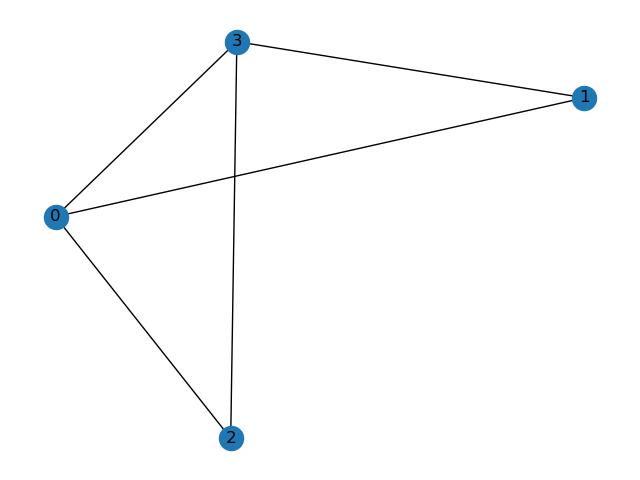
\includegraphics[width=8cm]{latex/Images/input_graph.png}
    \caption{Example input graph. \textcolor{red}{TODO: change to triangle free planar graph}.%TODO:
    }
    \label{fig:input_graph}
\end{figure}

\begin{figure}[H]
    \centering
    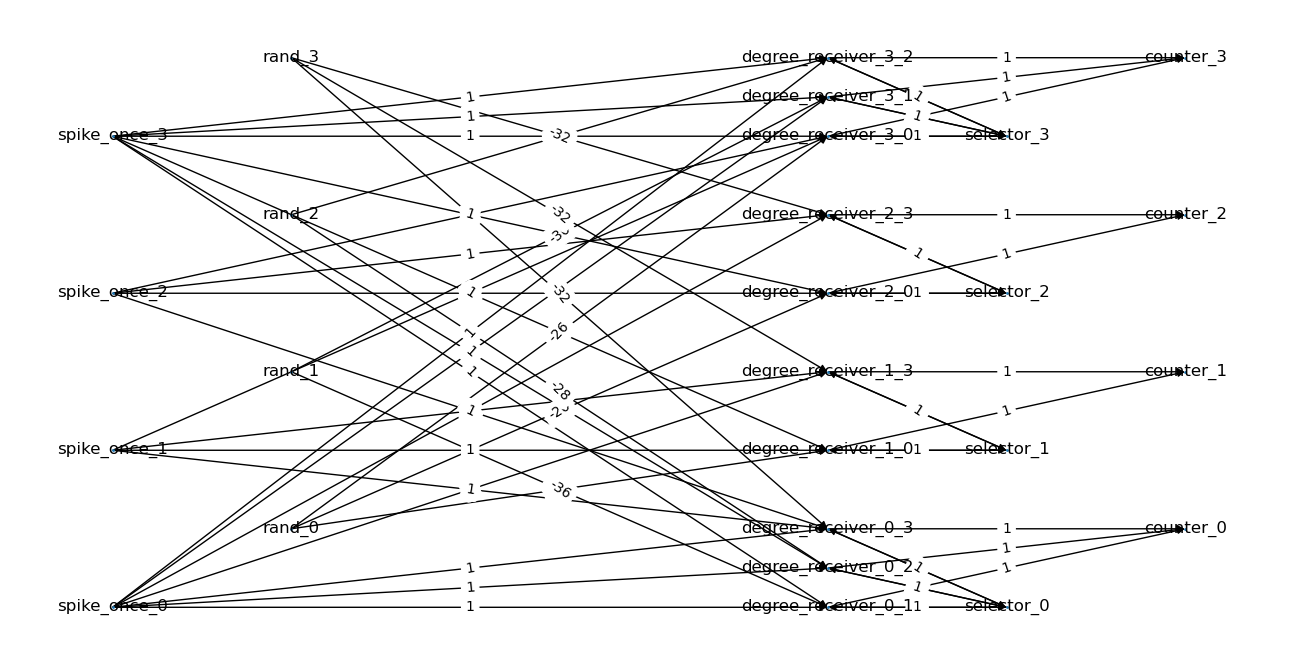
\includegraphics[width=8cm]{latex/Images/structured_graph.png}
    \caption{Example SNN encoding of algorithm to approximate MDS on the input graph of \cref{fig:input_graph}. This module is connected in series where the mark counter neuron takes up the role of spike\_once neuron in the next round of the approximation algorithm. For a more detailed description of the SNN implementation the reader is referred to Diehl et al., or to the source code documentation \cite{}. %TODO: include citation. %TODO: update to match updated input graph.
    }
    \label{fig:encoded_snn}
\end{figure}

This SSN implementation of the MDS approximation algorithm is onwards referred to as the default network. This default network is then enhanced with strategically placed redundant neurons that are inhibited by the default network neurons. Next, space radiation damage is simulated on the Loihi 2 in the form of random neuron deaths. This neuron death implies a neuron is removed from the SNN, and it can occur to both the default network and the redundancy neurons. If a default network neuron dies, the inhibition to the redundant neuron should be removed, causing the SNN to use the alternative neural pathway to recover from this damage.

\subsection{Hardware}\label{subsec:hardware}
Since at the time of writing no single-event effect (SEEs) propagation mechanisms are identified for space radiation exposure on the Loihi 1 \& 2 chips, a high-level software simulation of these single-event effects is performed. This is done by assuming the non-neuromorphic components of the chips are performing nominally, and that the SEEs propagate from for example transient bit-flips towards neuronal and synaptic parameter changes. The first assumptions may be accurate if local radiation hardening and redundancy is applied to the non-neuromorphic components. Weight and/or energy saving could be a motivation to apply these radiation counter-measures sparsely. The second assumption is based on the digital nature of the components that make up the neural components of the Loihi. The components that make up the neural compartments and synapses of the Loihi are visualised in \cref{fig:loihi_micro_architecture}.
\begin{figure}[H]
    \centering
    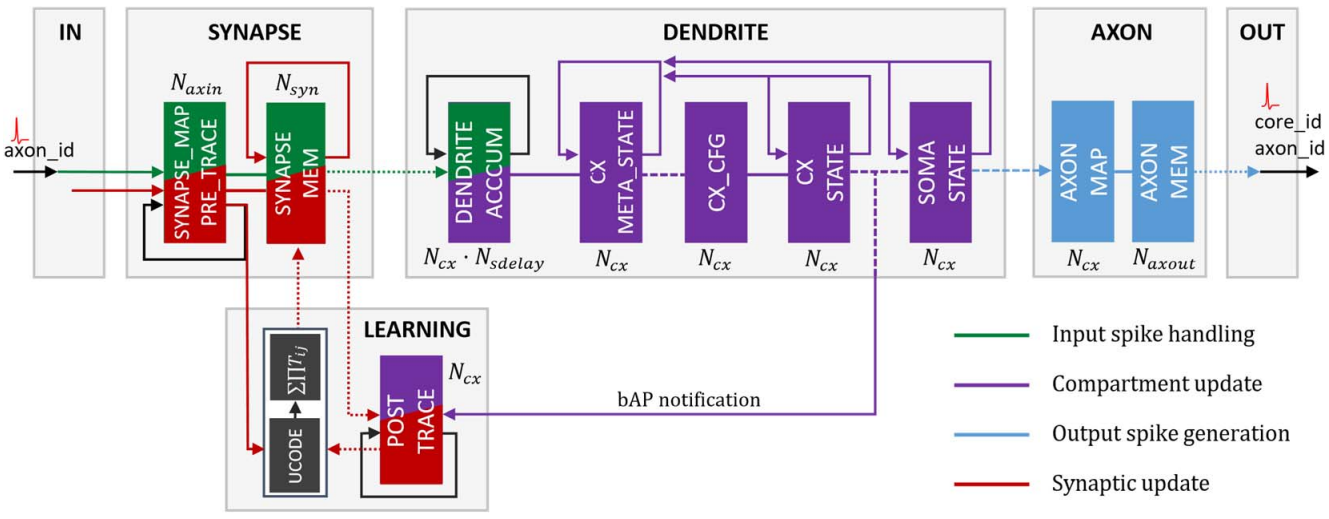
\includegraphics[width=8cm]{latex/Images/loihi_micro_architecture.png}
    \caption{Core Top-Level Microarchitecture of the Loihi chip. The SYNAPSE unit processes all incoming spikes and
    reads out the associated synaptic weights from the SRAM memory \cite{}%https://redwood.berkeley.edu/wp-content/uploads/2021/08/Davies2018.pdf
    .}
    \label{fig:loihi_micro_architecture}
\end{figure}



\subsection{Testing}\label{subsec:testing}
To test whether the brain adaptation implementations are successful, \textcolor{red}{three/one} brain adaptation implementations are compared to a baseline without brain adaptation and among each other. 

% TODO: verify subsubsections are allowed.
\subsubsection{Metrics}\label{subsubsec:metrics}
The metrics of the comparison are:
\begin{enumerate}
    \item \textit{Radiation Robustness} - a score from 0 to 100\% indicating the ratio of successful solution generation on random input graphs.
    \item \textit{Neuronal \& Synaptic Overcapcity} - a score from 0 to $n$\% indicating the ratio of redundant neurons and synapses with respect to the original implementation without adaptation implementation. % TODO: consistent default network naming see method/intro.
    \item \textit{Energy Efficiency} - the number of spikes consumed by implementations.
    \item \textit{Time complexity} - the theoretical time complexity required for network initialisation and adaptation.
    \item \textit{Space Complexity} - the theoretical space complexity required for network initialisation and adaptation.
\end{enumerate}

\subsubsection{Simulated Radiation Damage}\label{subsubsec:simulated_radiation_damage}
The following radiation damage is simulated:
\begin{enumerate}
    \item Neuron death.
    \item \textcolor{red}{Synaptic death.}
    \item \textcolor{red}{Neuron property changes in: $\delta u,\delta v, bias,vth$.}
    \item \textcolor{red}{Synaptic property changes in: $sign,weight$.}
\end{enumerate}

\subsubsection{Brain Adaptation Mechanisms}\label{subsubsec:brain_adaptation_mechanisms}
The tests are performed on the following brain adaptation implementations:
\begin{enumerate}
    \item \textcolor{red}{An Neumann monitoring module that scans the entire SNN network probing its behaviour, and re-routing broken neurons and/or synapses to redundant neurons.}
    \item Intelligently designed redundancies of inhibited neurons that automatically take over from deceased neurons.
    \item \textcolor{red}{A rate-coding frequency adaptation to reduce the relative impact of radiation induced spike omission in a subnetwork of the complete SNN implementation of the MDS approximation.}
\end{enumerate}